\scanpage{73}
% archive sheet number: 72

\diagram{\begin{tikzcd}\underline{G}(k\prime) \arrow[r,harpoon,thick] & \underline{G}(k)\ .\end{tikzcd}}
Ce dernier rend commutatif \inserted{(mod isomorphisme canonique)} le diagramme
\diagram{\begin{tikzcd}[ampersand replacement=\&,column sep=large,row sep=large]
\underline{G}(k\handwritten{'}) \handwritten{\arrow[r]} \handwritten{\arrow[d,draw=none,"{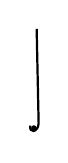
\begin{tikzpicture}[x=1cm,y=1cm,baseline=0cm]\draw[thick] (0,.7)--(.025,-.5)..controls (.02,-.62) and (-.1,-.63)..(-.08,-.53);\fill (-.035,-.56) circle (.035);\end{tikzpicture}}" description]} \& \underline{G}(k^{\deleted{\unsure{\prime|p}}}) \handwritten{\arrow[d,draw=none,"{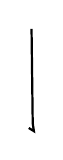
\begin{tikzpicture}[x=1cm,y=1cm,baseline=0cm]\draw[thick] (0,.7)--(.015,-.5)--(.03,-.6)--(-.035,-.56);\end{tikzpicture}}" description]} \\
\handwritten{\underline{\pi}_{p}}(k')\mathrm{x}\handwritten{[}G_m\handwritten{]}_{\underline{\unsure{\deleted{W}Q|\deleted{Q}W|\mathbb{Q}}}_p} \handwritten{\arrow[r]} \& \handwritten{\underline{\unsure{\pi|\Pi}}}_p(k)\mathrm{x}\handwritten{[}\underline{G}_m\handwritten{]}_{\underline{Q}_p}
\end{tikzcd}}
(i.e. on a, sur les catégories tannakiennes\deleted{, un} correspondantes, un dia\unsure{g|\deleted{r}g|\deleted{g}r}\unsure{\deleted{g}r|\deleted{r}g}amme comm\unsure{\deleted{y}u|\deleted{u}y}tatif à isomorphisme \inserted{can.} près).

Oubliant dans ce dernier les facteurs $\handwritten{[}\underline{G}_m\handwritten{]}$, on voit donc que $\underline{G}(k')\handwritten{\longrightarrow}\underline{G}(k)$ se factorise par la sous-\deleted{catégorie} gerbe de $\underline{G}(k)$ correspondant au sous-g\unsure{\deleted{o}r|\deleted{r}o}oupe fermé de $\handwritten{\pi}_1(k)$ image de $\handwritten{\pi}_1(k')$ ... A prouver:

\uline{Proposition} \handwritten{6.1.} Si $k'$ est une extension \deleted{finie} étale de $k$, alors l'homomorphisme de gerbes $\underline{G}(k')\handwritten{\longrightarrow}\underline{G}(k)$ est un \uline{monomorphisme} dont l'image est exactement la sous-gerbe ``ouverte'' définie ci-dessus. En particulie\unsure{\deleted{t}r|\deleted{r}t}, si $k'$ est une extension finie galoisienne de $k$, \deleted{on a une} de groupe de \raisebox{.4ex}{G}alois $g$, et on une suite exacte canonique de gerbes
\diagram{\begin{tikzcd}0 \arrow[r,thick] & \underset{\handwritten{\unsure{\mu|\pi|\Pi}}}{\underline{G}^{\deleted{\unsure{\prime|1}}}}(k\handwritten{\prime}) \arrow[r,thick] & \underline{G}(k) \arrow[r,draw=none,"{\begin{tikzpicture}[baseline=0cm,x=1cm,y=1cm]\draw[thick] (0,0)--(.6,0);\draw[thick] (.55,0)--(.55,-.04);\end{tikzpicture}}" description] & \handwritten{[}g\handwritten{]}_{\underline{Q}_p} \arrow[r,thick] & 0\ .\end{tikzcd}}
Cet énoncé devrait être formellement équivalent au suivant: $\operatorname{Spec}(k')\handwritten{\longrightarrow}\operatorname{Spec}(k)$ est un morphisme de descente effective pour la catégorie fibrée des $\mathrm{Fcriso}(L)$ sur des composés finis\inserted{$L$} de corps de car. $p$. La démonstration de ce dernier fait est $\handwritten{\pm}$ triviale.

\uline{Question} \handwritten{6.}\unsure{\deleted{1}\handwritten{2}|\handwritten{2}}\handwritten{.} A-t-on encore un énoncé analogue lorsqu'on suppose que $k'$ est une extension galoisienne de $k$ qui peut-être infinie ? Le cas le plus intéressant serait celui où $k'$est la clôture séparable de $k$, de sorte qu'on aurait un dévissage de $\underline{G}(k)$ \unsure{\deleted{a}e|\deleted{e}e}n
\diagram{\handwritten{(\unsure{6}.2.1)}\quad\begin{tikzcd}0 \arrow[r,thick] & \underline{G}(\handwritten{\bar{k}}\deleted{\vphantom{k}^{\unsure{\prime|1}}_{\unsure{s|3}}}) \arrow[r,thick] & \underline{G}(k) \arrow[r,thick] & \handwritten{\underline{\unsure{\pi|\Pi}}}_p(k) \arrow[r,thick] & 0\end{tikzcd}\quad\deleted{\unsure{?|;|x}}\ ;}
lorsque $k$ est parfait i.e. $\handwritten{\bar{k}}$ alg. clos, nous verrons que $\underline{G}(\handwritten{\bar{k}})$ ne dépend pas essentiellement de \handwritten{$k$. À}


